\documentclass{school-22.211-notes}
\date{May 14, 2012}

\begin{document}
\maketitle

\lecture{LWR Core Design}
This lecture combines the PWR core loading pattern lecture given for 22.211 on 05/14/2012 and the LWR core design lecture given for 22.39 on 10/02/12, 10/04/12. 


\topic{Objectives \& Constrain}
We have 3 objectives:
\begin{enumerate}
\item Meet the cycle length requirement provided by the finance people; typically 18-20 months. Assure core criticality for desired cycle operation. 
\item Maximize economy, for instance, BU. 
\item Assure plant availability: minimize vessel fluence, minimize back end costs. 
\end{enumerate}
and one constrain: Safety!
  \begin{itemize}
    \item Assure control for steady state operation behavior. 
    \item Assure reactivity control for safe shutdown margin or any other operational transients. 
    \item Assure acceptable core behavior in accidents. 
  \end{itemize}
Reactor physics interacts with other disciplines: 
\begin{itemize}
\item Thermal hydraulics: 
  \begin{itemize}
  \item Temperature field and fluid density affects core neutronics. 
  \item Temperature impact materials properties. 
  \item Balance of plant affects core operating conditions (and vise versa). 
  \end{itemize}
  For instance, the grid spacers are one of the most important factors, because the more fluid mixing we get, the better performance we get out of the core. 

\item Chemistry and materials: 
  \begin{itemize}
    \item Material interact: oxidation, corrosion, hydriding, PCI.
    \item Radiation environment changes materials properties and affects chemical interactions (radiolysis). 
  \end{itemize}
\end{itemize}


\clearpage
\topic{Design Tools: Lattice Code, Nodal Code}
Overview of reactor physics tools: 
\begin{enumerate}
\item Fuel pin performance code: FRAPTRAN, FALCON, etc. 
\item Lattice physics code: CASMO, TGBLA, PARAGON, etc. 
\item 3D steady state nodal code: SIMULATE, ANC, PANIC-x, etc.
\item Stability analysis tool: SIMULATE-3K, LAPUR, etc.
\item Transient system codes: RETRAN, RELAP, TRACE, etc.
\end{enumerate}
Overview of reactor physics methods:
\begin{enumerate}
\item Monte Carlo: 75 hours on 750 CPU to get 1\% 95/95 accuracy for the Hoogenboom/Martin problem. 

\item Discrete transport method (eg: SN method): 
  \begin{itemize}
    \item Lots of unknowns need to be solved from the energy groups, angles, axial mesh etc. For example, we can estimate the number of unknowns for a LWR core: (100 mesh/pin)(300 pins/assembly) (200 assemblies/core) (100 axial mesh) (100 energy groups) (1000 angles) = $6 \times 10^{13}$ unknowns. 
    \item Fine mesh transport takes roughly the same time with Monte Carlo. For instance, the best parallel transport `Grind time' SN code is Texas A\&M's PDT code which takes 300 nanosecond/unknown. Then assuming perfect scaling, the time required to solve a full core is, (6E13 unknowns)(3E-7 s/unknown)(20 fission source iterations/case) = 100,000 hours. Not to mention we haven't consider any feedback, cross section evaluations, boron search to criticality, equilibrium Xenon, control rod searches to criticality etc. 
    \item Hence discrete transport method has never been used for full core calculation. 
  \end{itemize}

\item Lattice code and nodal code (see Fig.~\ref{lattice-nodal-code}: we start with basic cross sections (for instance, from ENDF), generate multi-group library, perform an unit-cell calculation, perform a lattice calculation, and perform a whole core calculation. \textcolor{red}{unit cell calculation?}
\end{enumerate}
\begin{figure}[ht]
  \centering
  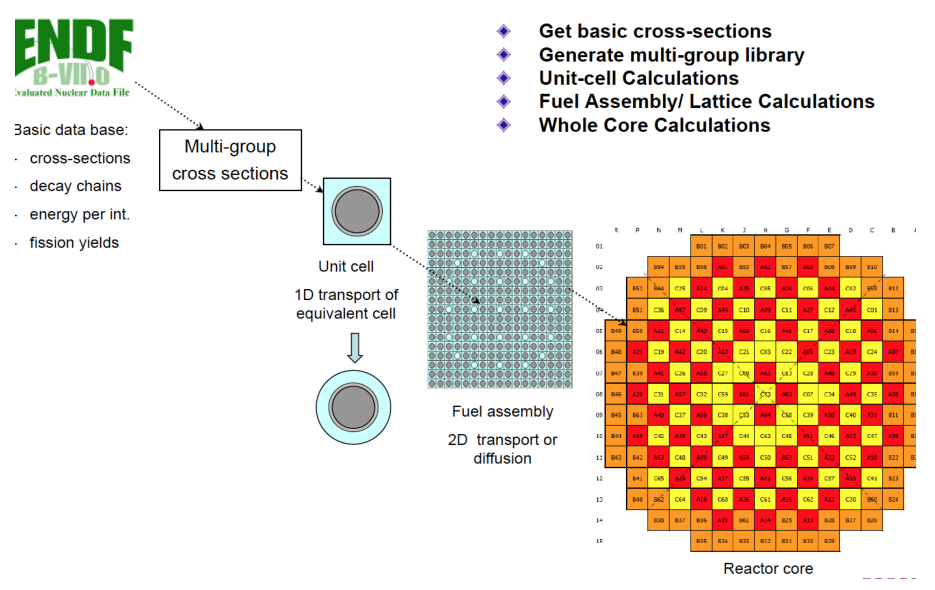
\includegraphics[width=4in]{images/design/lattice-nodal-code.png}
  \caption{Lattice Code Nodal Code Flowchart} \label{lattice-nodal-code}
\end{figure}



\subtopic{Lattice Code}
A lattice code calculation includes:
\begin{enumerate}
\item Pin spectrum calculation (energy domain). Lattice code solves for fine energy fluxes (1000s to 10,000s groups) with treatment of resolved resonances, and condense the cross sections to intermediate group cross sections (100s groups): 
  \eqn{ \sigma_{g} = \frac{\int_{E_{g-1}}^{E_{g}} \sigma(E) \phi(E) \dE  }{\int_{E_{g-1}}^{E_{g}} \phi(E) \dE}   }
\begin{figure}[ht]
  \centering
  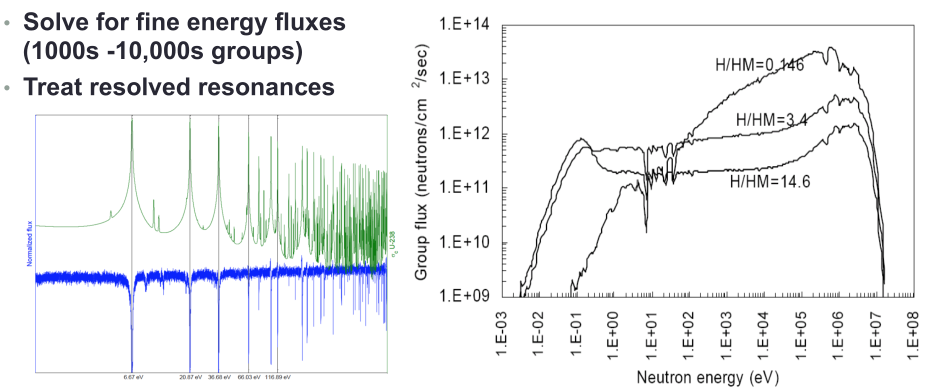
\includegraphics[width=4in]{images/design/lattice-energy.png}
  \caption{Lattice Code: Pin Spectrum Calculation} \label{lattice-energy}
\end{figure}

\item Intermediate group pin spatial calculation (spacial domain). Lattice code solves for radial distributions of nuclides and fluxes in each type of pin. For a lattice depletion code, we want to know is the pin-wise isotropic inventories vs. BU. Lattice code produces data library as a function of fuel BU, coolant density, fuel temperature, void, etc (so lattice code does not just solve for a steady state condition, it solves for about 2000 cases). 
\begin{figure}[ht]
  \centering
  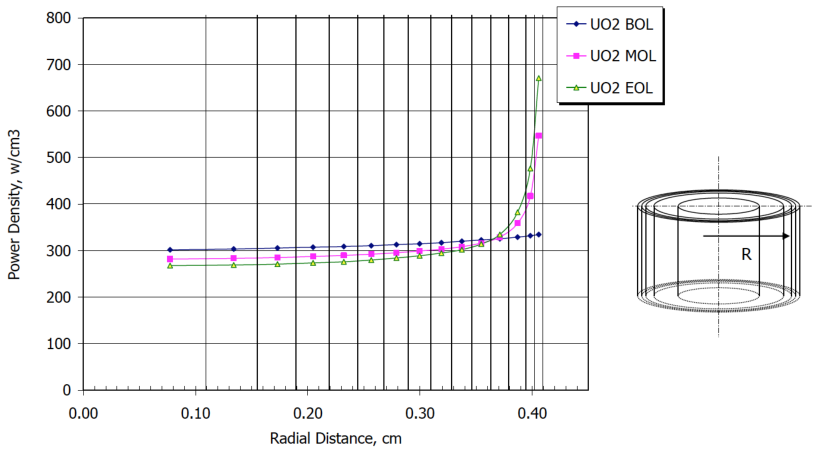
\includegraphics[width=4in]{images/design/lattice-space.png}
  \caption{Lattice Code: Pin Spatial Calculation} \label{lattice-space}
\end{figure}

\item Solve full assembly neutronics. Lattice code solves for pin-wise distribution of neutron fluxes (10-100 energy groups, homogenized pins). That's about 5000 spatial regions per assembly; MOC would take about 20 energy groups, 1000 angles, 0.05cm ray spacing. Then we compute $\keff$. 
\end{enumerate}

Comments: 
\begin{itemize}
\item For PWRs, $\rho$ vs. BU (with no burnable poisons) are just straight lines depending on enrichment. So long cycle and high BU we need high enrichment. So everyone is about 4\% enrichment in the US.  Corner pin power peaking: would be about 15\%. 
\begin{figure}[ht]
  \centering
  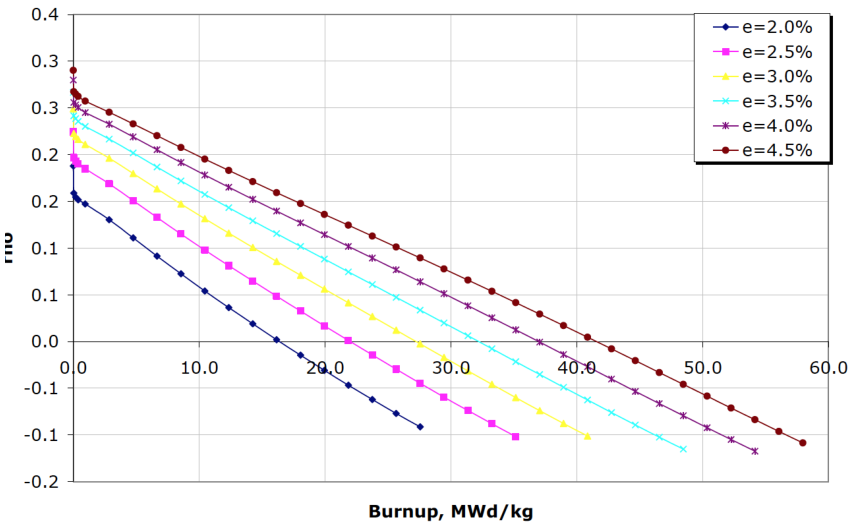
\includegraphics[width=4in]{images/design/lattice-rho-vs-BU.png}
  \caption{Lattice Code: PWR Assembly Reactivity vs. Burnup, Enrichment} \label{lattice-rho-vs-BU}
\end{figure}
\item Fission products absorption reduces reactivity of the fuel. 
\item U235 depletion significantly reduces reactivity as fissile inventory is reduced. 
\item Transmutation (particularly of U238) leads to complicated isotopic inventory. 
\item Pu239 production offsets part of the U235 reactivity depletion effects. 
\end{itemize}


\subtopic{Nodal Code}
A quick review of 3D advanced nodal codes: 
\begin{itemize}
\item 2D lattice transport/depletion calculation with approximated boundary conditions. 
\item 3D simulation using few group diffusion models with homogenization/condensation approximations. 
\item Fuel depletion on node-averaged basis: smooth intra-nodal spatial depletion representation. 
\item Local detail by superposition-based reconstruction. 
\item Pin conduction/bundle hydraulics: one characteristic pin and channel per bundle, no fluid cross flow between parallel channels, correlation-based heat transfer and void fraction models. 
\end{itemize}
Know the basic idea of the Transverse-integrate method: we transverse integrate 1D diffusion equation for the thermal group, approximate the source with 4th order Legendre polynomial, and solves for an analytical solution for the thermal group. Then we differentiate to get the net current at the interface, and use continuity of net currents/flux to get analytic expression for coupling. 




\clearpage
\topic{Uncertainty Analysis: Measurements}
We have a number of ways to determine the accuracy/uncertainty of core physics methods,
\begin{enumerate}
\item In-core flux mapping system: 58 instrumented locations and 61 (or 610) axial point measurements (through 58 tubes coming in from the bottom of the vessel). 
  \begin{itemize}
    \item Measurement should agree with simulation at core loading time to assure proper core loading. 
    \item Measurements will be performed monthly afterwards to assure compliance of power distribution with technical specifications (LHGR): verify peak LHGR with tech spec limits, verify pin/assembly burnup limits, determine 95/95 reliability factors for predictive models. 
    \item Zr spacers depress the flux because it displaces some water/moderator. 
    \item CMS codes provide very accurate power distribution, $\pm 300$pcm HFP core reactivity with depletion, and about 300pcm bias from CFP to HFP reactivity (Doppler, MTC) as see in Table~\ref{CMS-accuracy}. Notice TIP stands for Traversing In-core Probes, which are sensors inserted in the calibration tube of the LPRM assemblies to perform periodic calibration. Instrument tubes bend easily in BWRs, so BWRs tend to sample gamma for a more even distribution. 
      \begin{table}[ht]
        \centering
        \includegraphics[width=4in]{images/design/CMS-accuracy.png}
        \caption{BWR Predictive Accuracy of Nodal Codes} \label{CMS-accuracy}
      \end{table}
  \end{itemize}

\item Ex-core detector: calibrate based on flux maps, used to monitor core flux (power level) and axial power shape. 

\item HZP rod worth measurements. We solve IKE (given power extracted from the ex-core detector, we can back out $\rho (t)$ etc). Though when we are moving the rods, we cannot believe the point kinetics. That's why to perform a HZP rod worth measurement we have to wait: after a boron dilution, we move the rod in small number of steps, then wait. This takes more than 1 hours/rod, that's why dynamic rod worth calculation gets popular. Control rod worth has to be within 10\%.

\item Dynamic rod worth:  you pull rod out a little bit, then you drive your rod all the way in called banking (takes 2 minutes), then you pull the rod out again.  A subtle point here is that the power does not start to go up until the control rod is back in its criticality position (the power actually goes up a bit faster because of the delayed neutrons). Caution: flux should be high enough that statistics is reliable, but cannot be too high that the reactor goes critical.  See Section~\ref{dynamic-rod-worth} for more details. 
\end{enumerate}
Side note: Westinghouse designs have 228 notches in a control rod, CE has 100 notches. 


\clearpage
\topic{BWR Core Design} 
\subtopic{Lattice Design}


\subtopic{Core Loading Patterns}



\subtopic{Rod Patterns}



\subtopic{Thermal Margins}




\subtopic{Operational Analysis}



\subtopic{Safety Analysis}






\topic{PWR Core Loading Pattern Optimization}
Reference: Turinsky's `Core Isotopic Depletion and Fuel Management' in \textit{Handbook of Nuclear Engineering}, Springer (2010). 


Objectives
\begin{itemize}
\item Limit on power peaking. 
\item Increased margins to thermal limits (CHF, T$_{\mathrm{fuel}}$. 
\item Maximize economics. 
\end{itemize}
The fundamental tradeoff is between economics (maximize energy) and minimize safety risks (minimize peaking):
\begin{itemize}
\item Maximize energy: maximize EOC reactivity, maximize cycle length, maximize fuel burnup. 
\item Minimize peaking: minimize maximum enthalpy rise hot-channel factor F$_{\Delta H}$, minimize heat flux hot-channel factor. 
\end{itemize}


Loading Pattern Problem: 
\begin{enumerate}
\item Out-in: most burned on the inside. good economics, bad peaking factor. 
\item In-out: most burned on the outside. good peaking factor, bad economics.
\item Ring of fire: from outside to inside less fresh, except a ring of burned one near the out-side most. 
\end{enumerate}
A LP problem is, 
\begin{itemize}
\item is a nonlinear, mixed-integer problem (so no derivatives).
\item is inherently a multi-objective problem. 
\item is highly constrained. 
\item has disjoint feasible regions.
\item has an extremely large decision space. 
\end{itemize}
Stochastic optimization schemes are only real options, 
\begin{enumerate}
\item Simulated annealing.
\item Genetic algorithms.
\item Swarm intelligence (ant colony, particle swarm, etc). 
\end{enumerate}
Casting the Objectives: A common way for using multiple objectives is the \hi{augmented (weighted) objective}. Example for $k, p$: 
\eqn{ f(k,p) = (1.5 - p) - 100 H (1.15 - k) }
This is an easy way to to include constrains as penalties. A better approach would the Pareto optimal which is not covered in this lecture (Ask stephano for questions). 

\textbf{Simulated Annealing}: The physical process of annealing means bringing metals to a high temperature and let it cool slowly; if it cools slowly enough eventually it would get to its minimum energy. 
\begin{algorithm}
  \begin{algorithmic}
    \STATE Intialize $x, C_0, L_0$.  $k=0$. 
    \WHILE{not converged} 
    \STATE do 
    \ENDWHILE
  \end{algorithmic}
  \caption{Basic Simulated Annealing Algorithm}
\end{algorithm}
The key feature is 


\textbf{Genetic Algorithm}
\begin{algorithm}
  \begin{algorithmic}
    \STATE Create and evaluate an initial population of $N$ chromosomes.
    \WHILE{not converged} 
    \STATE Select $n$ chromosomes to reproduce (crossover); 
    \STATE Crossover and/or Mutate chromosomes;
    \STATE Replace $n$ least fit chromosomes with $n$ offsprings;
    \STATE Evaluate the population.
    \ENDWHILE
  \end{algorithmic}
  \caption{Basic Genetic Algorithm}
\end{algorithm}

\begin{enumerate}
\item  Selection criteria: survival of the fittest. 
  \begin{enumerate}
  \item Proportinal selection, Russian-Roulette. 
  \item 
  \end{enumerate}

\item Crossover: breeding patterns. This type of problem is called ordering problems: we have finite number of something that need to be conserved in the crossover. A typically way to do it is the Heuristic Tie-Breaking crossover: 

\item Mutation: add a bit of local refinement to the global scopes of GA. 

\item Replacement: 
  \begin{enumerate}
    \item Delete all (generational): replace all $N$ parents with $N$ offspring.    \item Steady state: replace some subset of $n$ parents with or without avoiding duplication.
  \end{enumerate}
\end{enumerate}



\textbf{Summary}
Comparison between SA and GA:
\begin{itemize}
\item SA is simpler to understand. SA is harder to parallelize (becase at each temperature you are making up a $L$ that depends on the previous steps). 
\item GA is natural for true `multiobjective' optimization. GA is trivial to parallelize. 
\item Both are heuristic and need some tuning. Both can be improved with hill-climbing heuristics (eg, greedy exhaustive single binary swaps). 
\end{itemize}
Once you put the most burned cores on the outside-most ring, how the inside pattern does not affect the cycle length anymore because the power on the outside is so small. But the peaking power is very sensitivie on the inner pattern. 
\end{document}
